\section{Echtzeitvisualisierung und OpenGL}
\subsection{Geschichte}
OpenGL entstand ursprünglich aus dem von Silicon Graphics (SGI) entwickelten IRIS GL. Im sogenannten Fahrenheit-Projekt versuchten Microsoft und SGI ihre 3D-Standards zu vereinheitlichen, das Projekt wurde jedoch wegen finanzieller Schwierigkeiten auf Seiten von SGI abgebrochen.

Der OpenGL-Standard wird vom OpenGL ARB (Architecture Review Board) festgelegt. Das ARB existiert seit 1992 und besteht aus einer Reihe von Firmen. Stimmberechtigte Mitglieder sind die Firmen 3DLabs, Apple, AMD/ATI, Dell, IBM, Intel, Nvidia, SGI und Sun (Stand Nov. 2004). Weiter mitwirkende Firmen sind Evans and Sutherland, Imagination Technologies, Matrox, Quantum3D, S3 Graphics, Spinor GmbH, Tungsten Graphics, und Xi Graphics. Microsoft, eines der Gründungsmitglieder, hat das ARB im März 2003 verlassen.

Neue Funktionen in OpenGL werden meist zuerst als herstellerspezifische Erweiterungen eingeführt und gehen dann den Weg über herstellerübergreifende Erweiterungen und ARB-Erweiterungen zu Kernfunktionalität. Dies erlaubt es, neueste Möglichkeiten der Grafikhardware zu nutzen und dennoch OpenGL abstrakt genug zu halten.

Quelle: https://de.wikipedia.org/wiki/OpenGL
\subsection{GL-Pipeline}
Eine Computergrafik-Pipeline besteht im Wesentlichen aus den folgenden Schritten:
\begin{figure}[H]
    \centering
    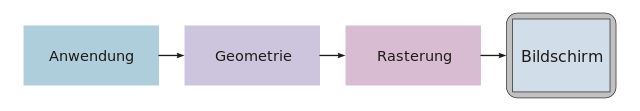
\includegraphics[width=1.0\textwidth]{images/cgpipeline_grob.png}
    \caption{Computergrafik-Pipeline}
    \label{fig:gimbal+lock}
\end{figure}

Eine solche Pipeline wird auch von OpenGL implementiert. Es besteht jedoch die Besonderheit, dass die Geometrie und die  Rasterung in Hardware realisiert ist und man durch kleine Programme, sogenannte Shader, auf diese Hardware zugreifen und Manipulationen vornehmen kann beziehungsweise seit OpenGL 2.0 sogar muss.



\subsubsection{Geometrie}
Die Geometrieverarbeitung   besteht aus der Hintereinanderausführung der folgenden affinen/homogenen Abbildungen und Algorithmen:
\begin{figure}[H]
    \centering
    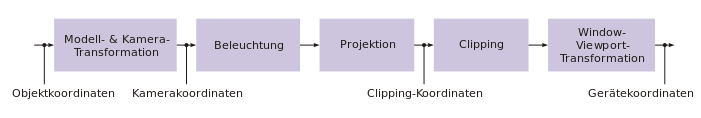
\includegraphics[width=1.0\textwidth]{images/cgpipeline.png}
    \caption{Geometrie-Pipeline}
    \label{fig:gimbal+lock}
\end{figure}

\subsubsection*{Modell und Kameratransformationen}
Die Transformationen von Objektkoordinaten in das Kamerakoordinatensystem werden durch affine Transformationen beschrieben, welche durch Multiplikation durch homogene $4 \times 4$-Matrizen realisiert werden. 

\subsubsection*{Projektion}
Die Projektion  wird durch  Matrizen  ähnlich der Projektionsmatrix $K_{persp_{xy}}$ und   $K_{orth_{xy}}$ aus Abschnitt 1.2.1 realisiert.
Es werden jedoch noch  Translationen, Rotationen Stauchungen dazwischengeschaltet, die ebenfalls als $4 \times 4$-Matrizen realisiert werden können und mit denen diese Marine multipliziert werden.  Man erreicht damit, dass der Kegelstumpf zwischen der forderen Projektionsebene, auch 'nearplane' genannt,  und der hinteren Ebene, auch 'farplane' genannt, in den $[-1,1] \times [-1,1] \times [-1,1] $ Würfel abgebildet wird.   
\begin{figure}[H]
    \centering
    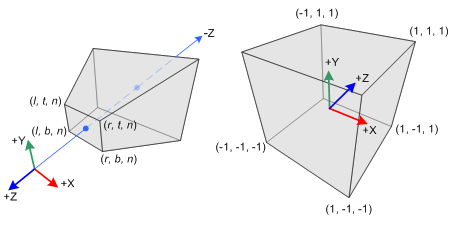
\includegraphics[width=1.0\textwidth]{images/gl_projectionmatrix01.png}
\end{figure}

Die Multiplikation all diese Matrizen wird auch die MODEL-VIEW-PROJECTION-MATRIX genannt. 

\subsubsection*{Windows-Viewport-Transformation}
Zuletzt müssen die zweidimensionalen Punkte noch mit Hilfe einer zweidimensionalen affine Transformation  in das Koordinatensystems des Anzeigenfensters auf dem Ausgabegerät transformiert werden. 
Diese Transformation wird auch Windows-Viewport-Transformation genannt.

\subsubsection{Rasterung}
\begin{figure}[H]
    \centering
    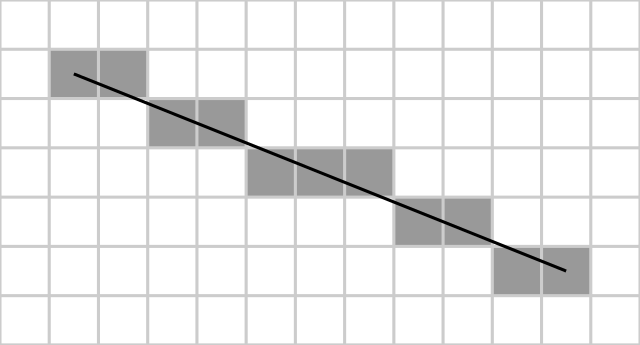
\includegraphics[width=1.0\textwidth]{images/bresenham.png}
    \caption{Bresenham Algorithmus}
    \label{fig:gimbal+lock}
\end{figure}
Als Rasterung bezeichnet man das transformieren kontinuierlicher, zweidimensionaler Daten auf diskrete Pixel.
Anhand der gegebenen Daten muss also entschieden werden, welche Farbe ein Pixel des Ausgabegerätes erhält.
Wir haben also eine Funtkion $Frame-Buffer: \mathbb{N} \times \mathbb{N} \to Farbe$.
Im Bereich Echtzeitvisualisierung  sind alle gängigen Rasterverfahren für Dreiecke und andere primitiven  im wesentlichen Abwandlungen und Weiterentwicklungen  von Algorithmen, die von  Bresenham eingeführt wurden. Wir wollen uns den Bresenham Algorithmus für Linien dazu exemplarisch anschauen.


Das Rastern erzeugt oft harte, kantige und ausgefranzte Übergange. Diese Effekte bezeichnet man auch als Aliasing. Algorithmen, die diesen Aliasing-Effekten entgegenwirken nennt man auch 
Antialiasing. 
\begin{figure}[H]
    \centering
    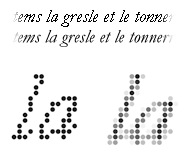
\includegraphics[width=0.5\textwidth]{images/Antialiasing.png}
    \caption{Eine Schrift mit und ohne Antialiasing}
    \label{fig:gimbal+lock}
\end{figure}


\subsubsection*{Sichtbarkeitsprobleme}
\begin{Definition}[Clipping]
\end{Definition}

\begin{Definition}[z-Buffer]
Der Z-Buffer enthält für jedes Pixel $(u,v)$ nach der Rasterung  einen Wert zwischen $-1$ und $1$. Dieser Wert  ist der Abstand zum nächsten Punkt eines Polygons  in Clipping-Koordinaten von diesem Pixel auf der Projektionsebene.  Wir haben somit eine Funktion
\begin{align*}
Z-Buffer : \mathbb{N} \times \mathbb{N} \to [-1,1]  \; .
\end{align*}
\end{Definition}

\begin{figure}[H]
    \centering
    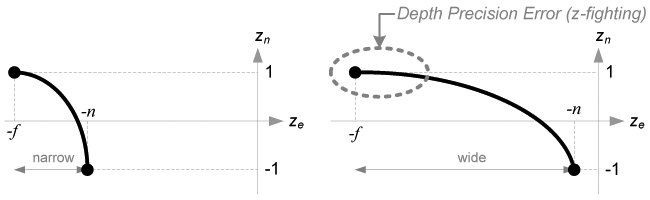
\includegraphics[width=1.0\textwidth]{images/gl_projectionmatrix_zbuffer_1.png}
    \caption{Z-BUFFER-WAR}
\end{figure}



\begin{Algorithmus}[z-Buffer Algorithmus]
Setze Alle Einträge im Z-Buffer auf 1 (Hintergrund).
Setze alle Einträge im Framebuffer auf die Hintergrundfarbe. \\
$\forall$ Polygone P: \\
begin: \\
Transformiere das Polygon in Clipping-Koordinaten. \\
Transformiere das Polygon in Rasterkoordinaten. \\
$\forall$ erhaltenen Pixel (u,v): \\
begin: \\
$pz := $Z-Koordinate des Polygons in Clipping-Koordinaten zum entsprechenden Pixel \\
$zz:=$ Eintrag im Z-Buffer für das Pixel $(u,v)$ \\
if $pz < zz$: \\
begin: \\
$Z-Buffer(u,v) := pz$ \\
$Frame-Buffer(u,v) := Farbe(P,(u,v))$ \\
end \\
end \\
end

\end{Algorithmus}





\subsection{Lokale Beleuchtungsmodelle}
\subsubsection{Ideale Reflexionen und Lichtbrechungen}
\subsubsection{Lambert  Modell}
\subsubsection{Phong Modell}

\subsection{Texturen und UV-Mapping}
\subsection{Shaderprogrammierung und standard Algorithmen}
\subsubsection{Syntax und Funktionsumfang}
\subsubsection{Flat  shading}
\subsubsection{Phong  shading}
\subsubsection{Bumpmapping}
\subsubsection{Displacementmapping}
\subsubsection{Shadowmap}


\subsection{WebGL}
